Having established a solid background of crop yield prediction with deep learning models, it is time to review the contributions of the publications selected for this dissertation. The objective of this dissertation is to probe and answer the research questions outlined in Chapter~\ref{ch:introduction}. RQ1 and RQ2 provide a suitable line of division for the selected publications. The feasiblity of spatial and spatiotemporal deep learning models in-season yield prediction with high resolution remote sensing data is explicitly studied in publications [I] and [IV]. In both, the models are designed, trained and evaluated from scratch to perform intra-field crop yield prediction with UAV-based data, within a growing season. Furthermore, [II] uses the model of [I] in a case study to frame the use of such models in a farming DSS. Two remaining publications, [III] and [V], focus on data sources. In [V], the effects of additional data sources were evaluated by comparing crop yield estimation performance with a static model architecture from [I]. Publication [III], while taking a distinct approach in terms of the modelling technique used, focuses on the reliability of satellite-based remote sensing data.

This chapter focuses on the data, methods and results of the selected publications, leaving discussion of the results and methods to Chapter~\ref{ch:conclusions}. The chapter consists of two main sections and is constructed as follows. In the first section, the developments and evaluations of intra-field crop yield prediction models are described. The section begins by looking at CNN-based yield prediction with distinct point-in-time frames presented in [I]. A frame is a sub-area extracted from larger images. Next, the evaluation of the usability of the best model of [I] in the farming DSS context is presented in [II]. Lastly, the development and evaluation of multiple spatiotemporal deep learning models in [IV] to perform crop yield prediction using UAV-based data is described. The second section focuses on data evaluation. The general outline of [V] is first described, where the effects of varying the input data source configurations on crop yield prediction performance were studied. The process of using machine learning to evaluate satellite data reliability with regards to cloud canopy [III] is described last.


\section{Intra-field crop yield prediction}
\label{sec:crop-yield-prediction-results}

\subsection{Single input to single target}
\label{subsec:single-input-results}

In working towards an effective in-season crop yield predictor model for the northern climate, the effort in [I] was to develop a CNN based deep learning framework using UAV-acquired multispectral data. RGB and NDVI images were fed as input data. The best perfofming CNN configuration in terms of architectural composition and hyperparameters (parameters defining the training setup, was iteratively developed via a tuning process). 

The nine crop fields selected for this study are located in the vicinity of the city of Pori (61$^\circ$29'6.5''N, 21$^\circ$47'50.7''E). The total area of the fields was approximately 90 ha. The main crops grown in the fields were wheat and malting barley, however the model was trained over the fields without making a distinction between the crop type. Details of the fields, crops, imaging dates and corresponding growth phases are listed in Table \ref{tab:i-field-info}. Thermal times for each crop variety are taken from a \cite{Luke2017}. Sowing dates and imaging dates are used to calculate the growth phase as a fraction of the total thermal time for the crop variety. Images with dates prior to 1st of July form the early data set and the remaining images the late one. 

\begin{table}[ht]
    \scriptsize
    \centering
    \caption{Details of crops and their varieties sown in each of the 9 fields in 2017 (reproduced from [I]).}
    \label{tab:i-field-info}
    \vspace{0.3cm}
    \begin{tabular}{cccccccc}
    \hline
    \textbf{\makecell{Field\\\#}}			& \textbf{\makecell{Size \\ (ha)}}	& \textbf{\makecell{Mean yield \\ (kg/ha)}}  	& \textbf{\makecell{Crop\\(\textit{Variety})}}  & \textbf{\makecell{Thermal\\time}}		& \textbf{\makecell{Sowing\\date}}	& \textbf{\makecell{Imaging\\date}}	& \textbf{\makecell{Growth\\phase}}\\ 
    \hline
    1 & 5.96    & 5098  & \makecell{Wheat\\(\textit{Zebra})}   & 1052  & 10 May    & 17 Aug & 83 \% \\ 
    \hline
    \multirow{2}{*}{2}	& \multirow{2}{*}{10.26} & \multirow{2}{*}{6054} 	& \multirow{2}{*}{\makecell{Barley\\(\textit{Trekker})}}	& \multirow{2}{*}{979.7}	& \multirow{2}{*}{16 May} & 8 Jun & 15 \% \\ 
    \cline{7-8}
    & &	& & & & 27 Jul & 64 \% \\ 
    \hline
    \multirow{2}{*}{3}	& \multirow{2}{*}{2.97}	& \multirow{2}{*}{8971} 	& \multirow{2}{*}{\makecell{Barley\\(\textit{Trekker})}}	& \multirow{2}{*}{979.7}	& \multirow{2}{*}{17 May} & 8 Jun & 15 \% \\ 
    \cline{7-8}
    & &	& & & & 27 Jul & 64 \% \\ 
    \hline
    4 & 13.05 & 4673 & \makecell{Barley\\(\textit{RGT Planet})} & 982.2  & 15 May & 6 Jul & 42 \% \\ 
    \hline
    5 & 4.66 & 6482 & \makecell{Barley\\(\textit{Propino})} & 981.4 & 15 May & 15 Jun & 22 \% \\ 
    \hline
    6 & 7.29 & 6884 & \makecell{Barley\\(\textit{Propino})} & 981.4 & 15 May & 15 Jun & 22 \% \\ 
    \hline
    7 & 10.92 & 7568 & \makecell{Barley\\(\textit{Harbinger})} & 976.3 & 24 May & 6 Jul & 36 \% \\ 
    \hline
    \multirow{2}{*}{8}	& \multirow{2}{*}{15.28}	& \multirow{2}{*}{7585} 	& \multirow{2}{*}{\makecell{Barley\\(\textit{Trekker})}}	& \multirow{2}{*}{979.7}	& \multirow{2}{*}{18 May} & 1 Jun & 10 \% \\ 
    \cline{7-8}
    & &	& & & & 13 Jul & 49 \% \\ 
    \hline				
    \multirow{2}{*}{9}	& \multirow{2}{*}{18.86}	& \multirow{2}{*}{6991} 	& \multirow{2}{*}{\makecell{Wheat\\(\textit{KWS Solanus})}}	& \multirow{2}{*}{1065}	& \multirow{2}{*}{13 May} & 15 Jun & 21 \% \\ 
    \cline{7-8}
    & &	& & & & 6 Jul & 72 \% \\ 
    \hline
    \end{tabular}
    \end{table}

Multispectral data was acquired from these fields during the growing season of 2017. The data was collected with a single Airinov Solo 3DR (Parrot Drone SAS, Paris, France) UAV equipped with NIR-capable SEQUIOA (Parrot Drone SAS, Paris, France) sensor. The images of individual spectral bands were stitched together to form complete orthogonal RGB and NDVI rasters of distinct fields using the Pix4D software.

The harvest yield data was acquired during September 2017 using two distinct setups attached to the harvesters: Trimble (Sunnyvale, California, USA) CFX 750 and John Deere (Moline, Illinois, USA) Greenstar 1. The data was initially in vector data point format. The points were first filtered according to \cite{Tiusanen2017} to preserve only points corresponding to harvester speed between 2 and 7 km/h and yield between 1500 and 15000 kg/ha. Then the field-wise data was rasterized by interpolation using an exponential point-wise inverse distance algorithm.

The field-wise image data was then processed using a sliding window to extract geolocationally matched pairs of input RGB and NDVI image frames and frame-wise averaged crop yields as targets of predefined size from all the fields. The step of the applied sliding window was chosen to be 10 m according to the resolution of Sentinel-2 satellite data considering the possibility of using satellite data as an additional input to the network in future studies. In other words, frames having sides longer than 10 m share data with adjacent frames due to overlapping. The resolution of the UAV data was 0.3125 m/px or 32 px per 10 m. Square image frames with side lengths of 10m, 20 m and 40 m were considered. The number of extracted frames was approximately 15200 for each frame dimension. All nine fields were first split into overlapping data frames of sizes 10 m, 20 m and 40 m. A dedicated holdout test data set was then built from 15 \% of shuffled data frames; this data was never presented to the model during training. The remaining 85 \% of data frames were then used for training the models with $k$-fold cross validation. After the training phase of each model was completed, the test errors were calculated using the holdout test data set to validate the performance of the trained model. This process is illustrated in Figure \ref{fig:i-data-handling}. 

\begin{figure}[ht]
    \centering
    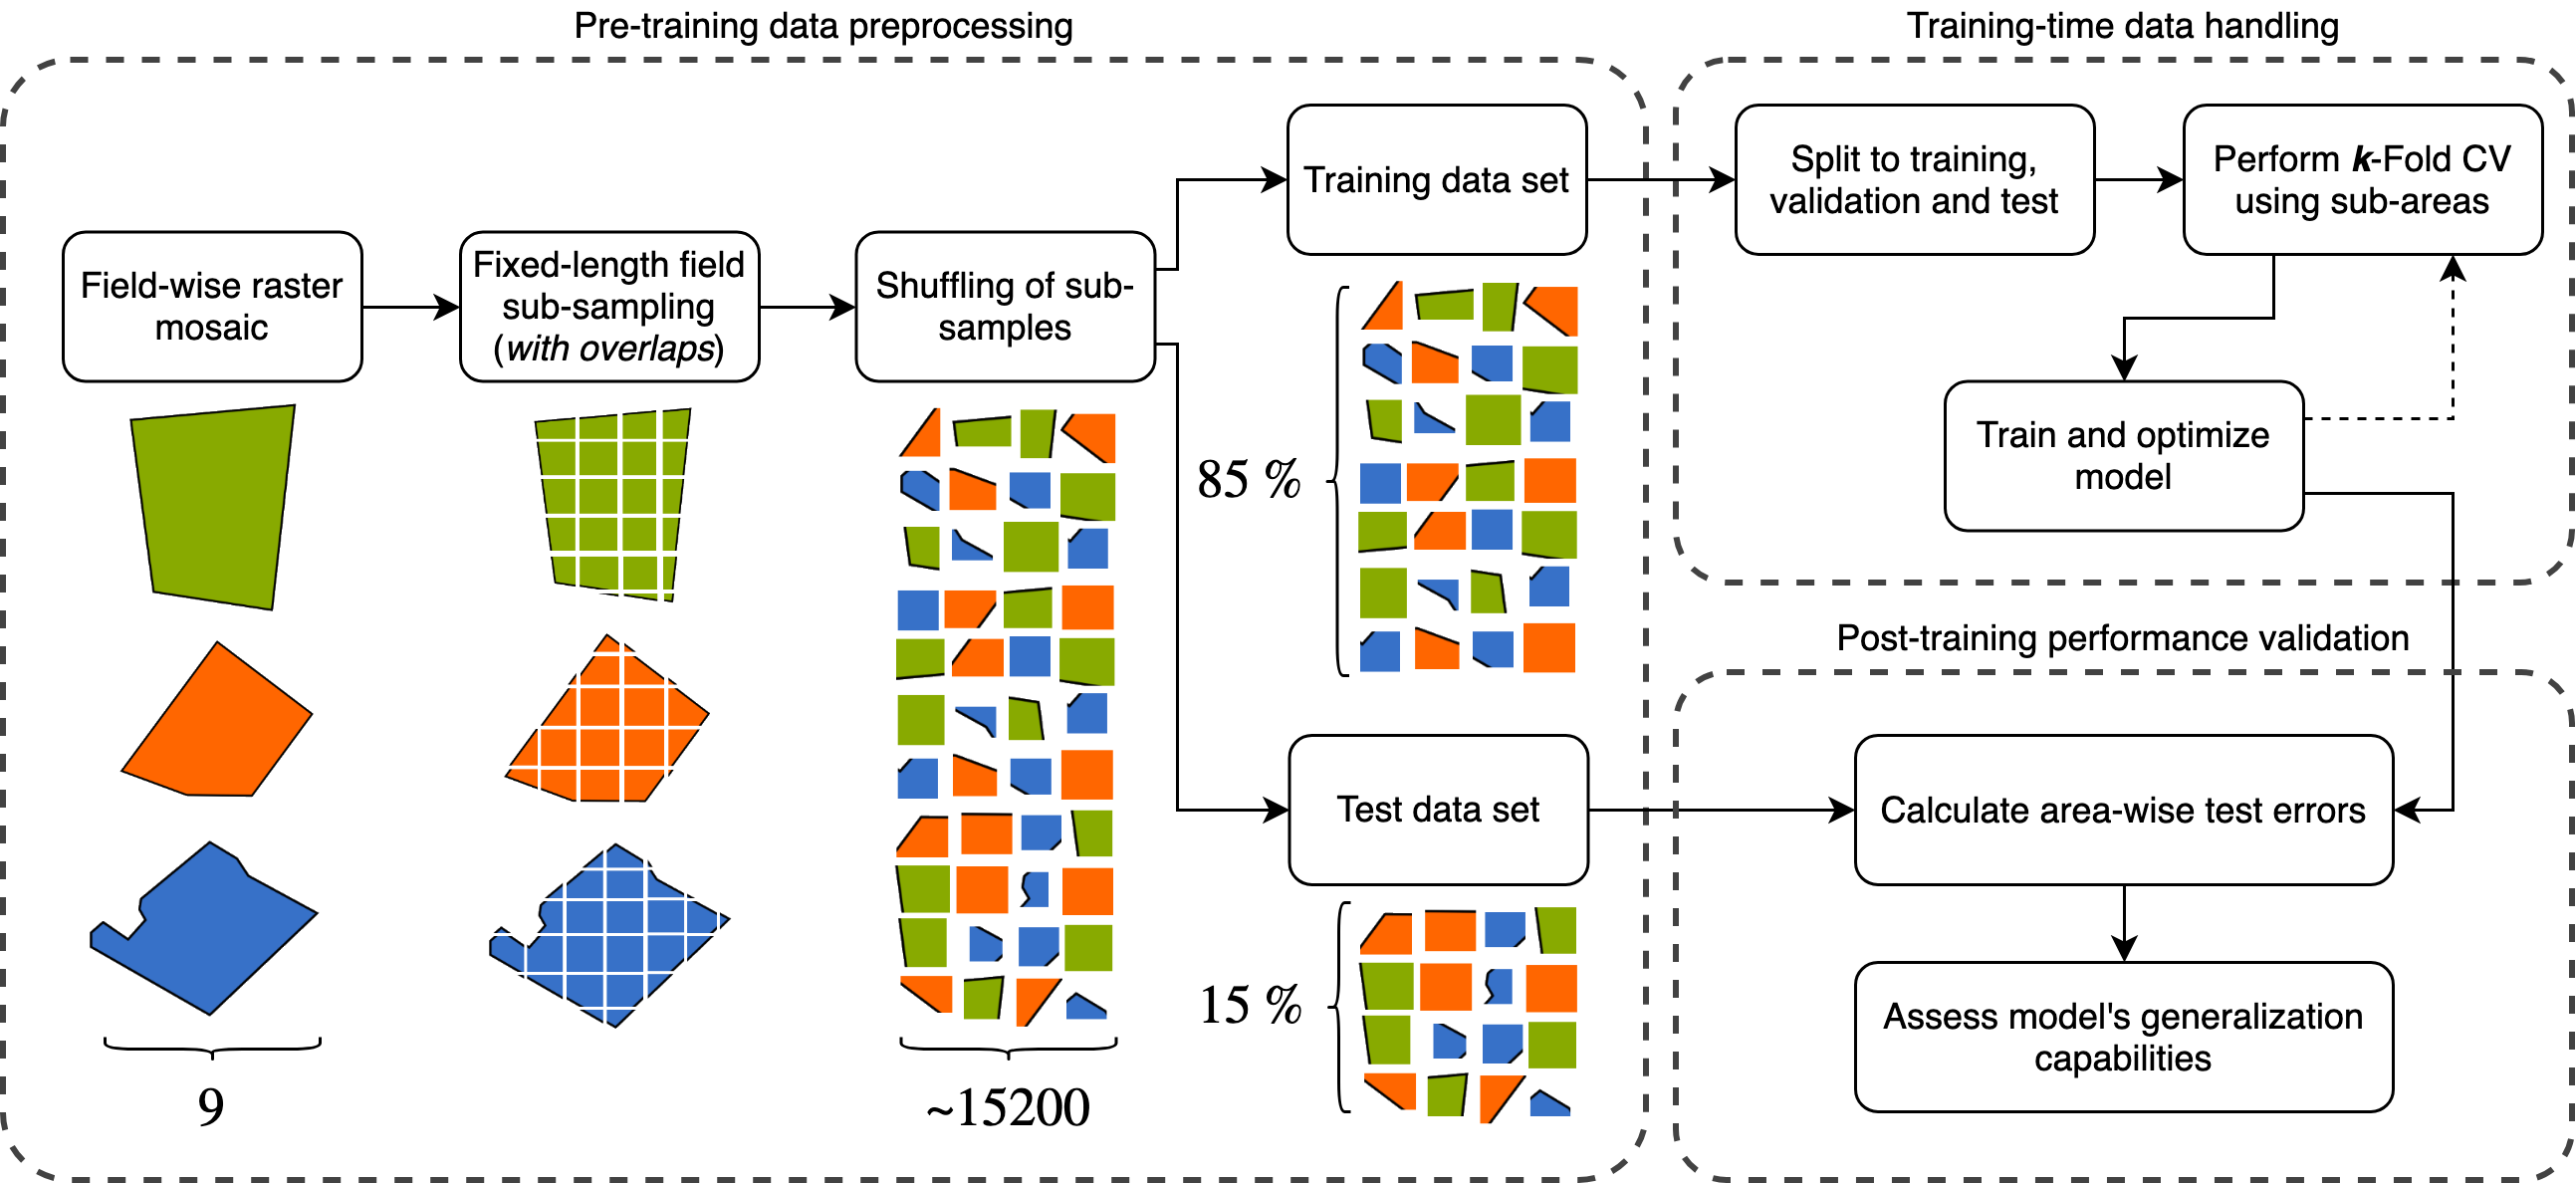
\includegraphics[width = \textwidth]{images/i-data-handling.png}
    \caption{The process of data preparation prior to and during training (reproduced from [I]).}
    \label{fig:i-data-handling}
\end{figure}

The basic architecture of the implemented CNN model follows closely the one reported in \cite{Krizhevsky2017a}. The general topology of the network is depicted in Figure \ref{fig:i-cnn}. The model was implemented using the PyTorch framework \cite{paszke2017automatic}. The model's inputs can be single-band or multi-band images ($B$) with varying dimensions ($D$). The network has at least two convolutional layers accompanied with two fully connected layers. The depth of the network is controlled by the number of intermediary convolutional layers. The last convolutional layer has 128 kernels while the intermediary layers have 64 kernels. Max pooling is applied only in the first and last convolutional layers so that the size of the data representation stays consistent when network depth is varied. The model uses non-overlapping pooling windows with pooling window size of 5 and a pooling stride matching the pooling window size. Pooling is applied only in the first and the last convolutional layers. Rectified linear units (ReLU) \cite{He2015} are used for layer-wise non-linear activation functions. This way our network is also scalable with respect to the number of layers. Two FC layers with 1024 neurons per layer are used to produce the final output from the CNN outputs.

\begin{figure}[ht]
\centering
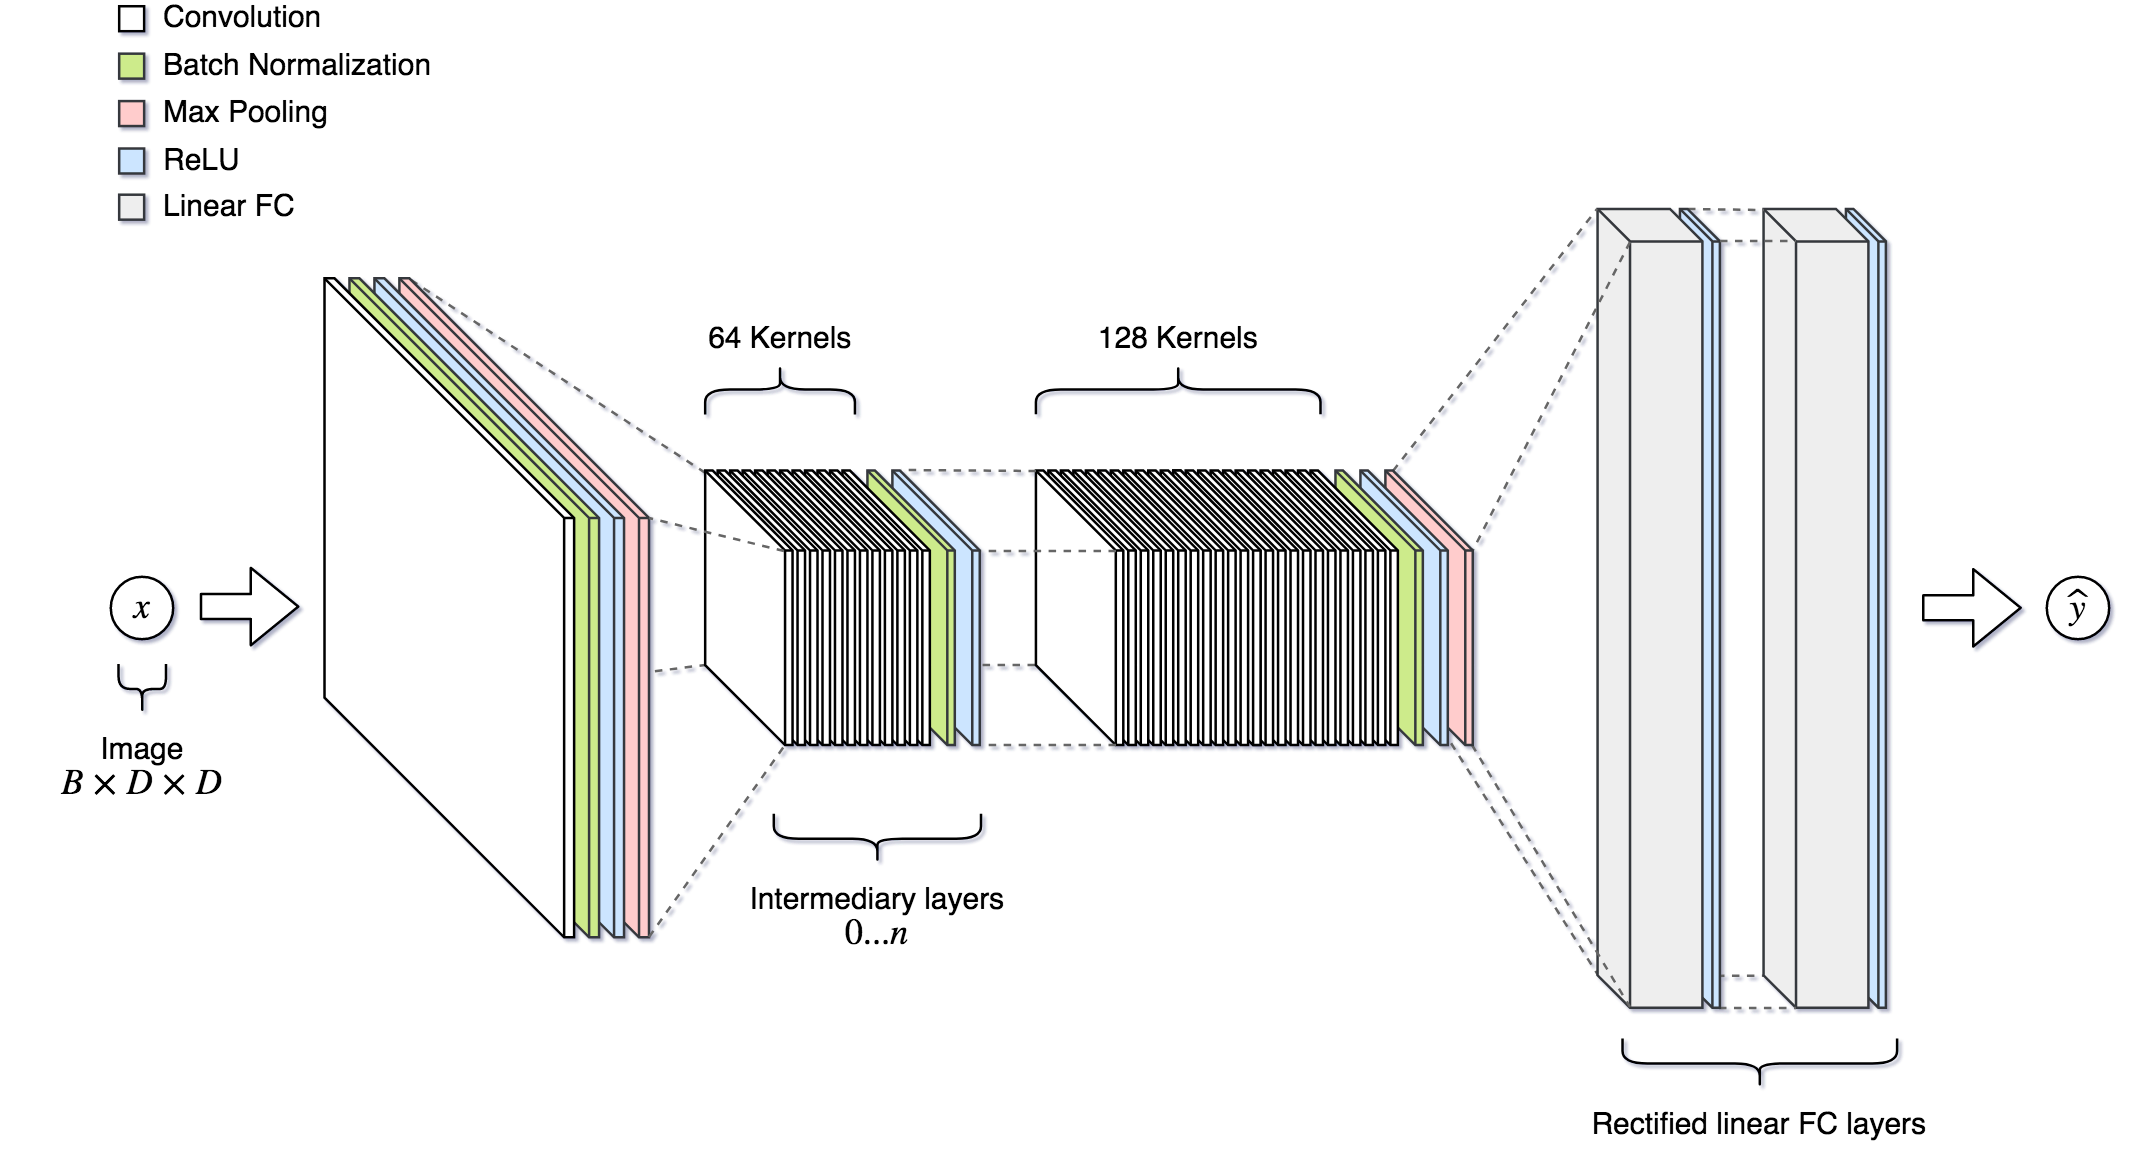
\includegraphics[width = \textwidth]{Images/i-cnn.png}
\caption{The overall topology of the implemented CNN (reproduced from [I]). }
\label{fig:i-cnn}
\end{figure}

Finding the optimal configuration of any deep learning network is an iterative process, where the model's parameters are initialized and tuned multiple times. The best training algorithm was evaluated among three options: Stochastic Gradient Descent with momentum (SGD-momentum) \cite{Bottou1998}, RMSprop \cite{Hinton2014} and Adadelta \cite{Zeiler2012} as suggested in \cite{Goodfellow-et-al-2016} and present in \cite{Karpathy2017}. Out of these, Adadelta performed the best. Optimizer parameters, such as learning rate, coefficient of using past gradients during backpropagation and weight decay, were tuned using random search \cite{Bergstra2012}. Other parameters were tuned by testing various values from predefined selections. These parameters were

\begin{itemize}
    \item input sample batch size (from $2^5$ to $2^{10}$)
    \item the number of intermediate convolutional layers (from 4 to 12)
    \item input data type (NDVI or RGB)
    \item frame side length (10m 20m or 40m)
    \item early stopping patience (from 10 to 50).
\end{itemize}

The lowest test set error of 484 kg/ha MAE and 8.8 \% MAPE was achieved using RGB data from the beginning of the growing season, i.e. pre-June images. R$^2$ score was 0.857. The best model consisted of six convolutional layers followed by two fully connected layers, using weight decay regularization with the coefficient being $10^{-3}$ and early stopping with patience of 50. The optimizer was also tuned, with the optimal values for learning rate and the coefficient adjusting the effect of past iterations' error corrections being $8 \times 10^{-3}$ and 0.58, respectively. The results show that the lowest test errors were achieved with the largest frame side length of 40 m. 

The best performing model was also utilized in a case study of six fields containing mostly barley, together accounting for 54.2 ha of land area and located near the city of Pori [II]. Imaging and yield acquisition methods were identical to [I], with some overlaps in the field-wise data. The crop yield prediction results indicate a consistent pattern of overestimating low yields and underestimating high yields. This is shown in Figure~\ref{fig:ii-FigurePallette}, where all values are absolute and in kg/ha. Over the six fields, the model attained 0.798 R$^2$, on average. Field-wise MAPE boxplots are depicted in Figure~\ref{fig:ii-boxplots}. 

\begin{figure}[htb]
    \centering
    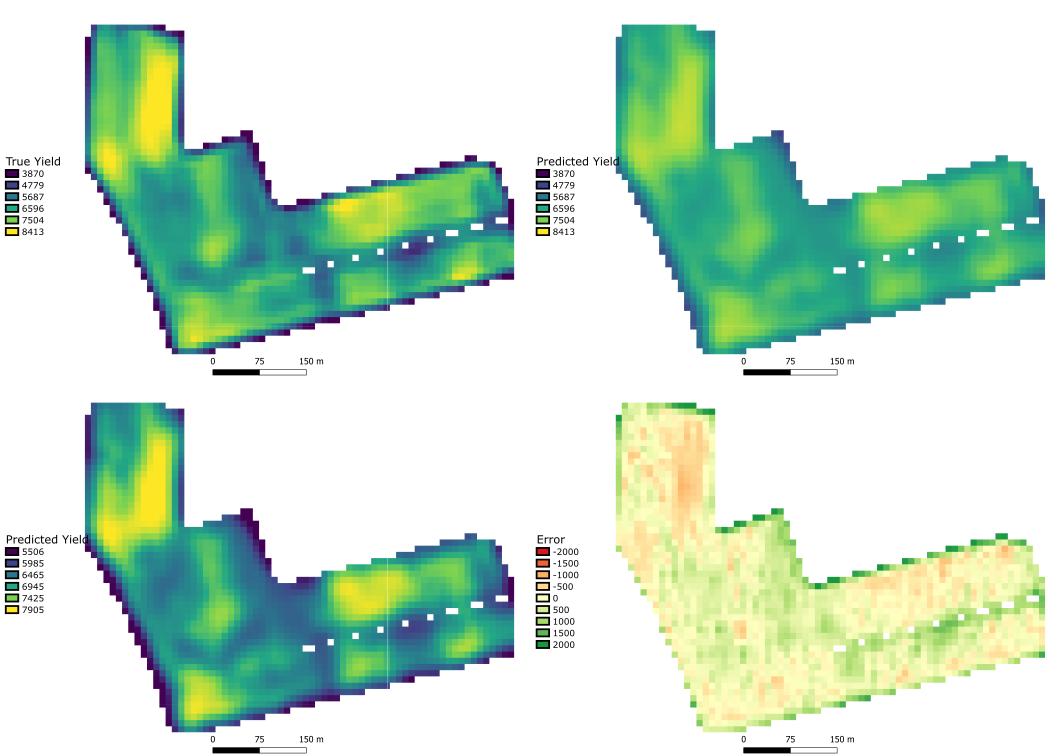
\includegraphics[width = \textwidth]{Images/ii-FigurePallette.png}
    \caption{Visualisation of the true and predicted yield of a field (reproduced from [II]). Images of true and predicted yields in the top row share a similar scale. Bottom left image is scaled to predicted values only. Bottom right image depicts the error between true and predicted yield. Units are in kg/ha.}
    \label{fig:ii-FigurePallette}
\end{figure}

\begin{figure}[htb]
    \centering
    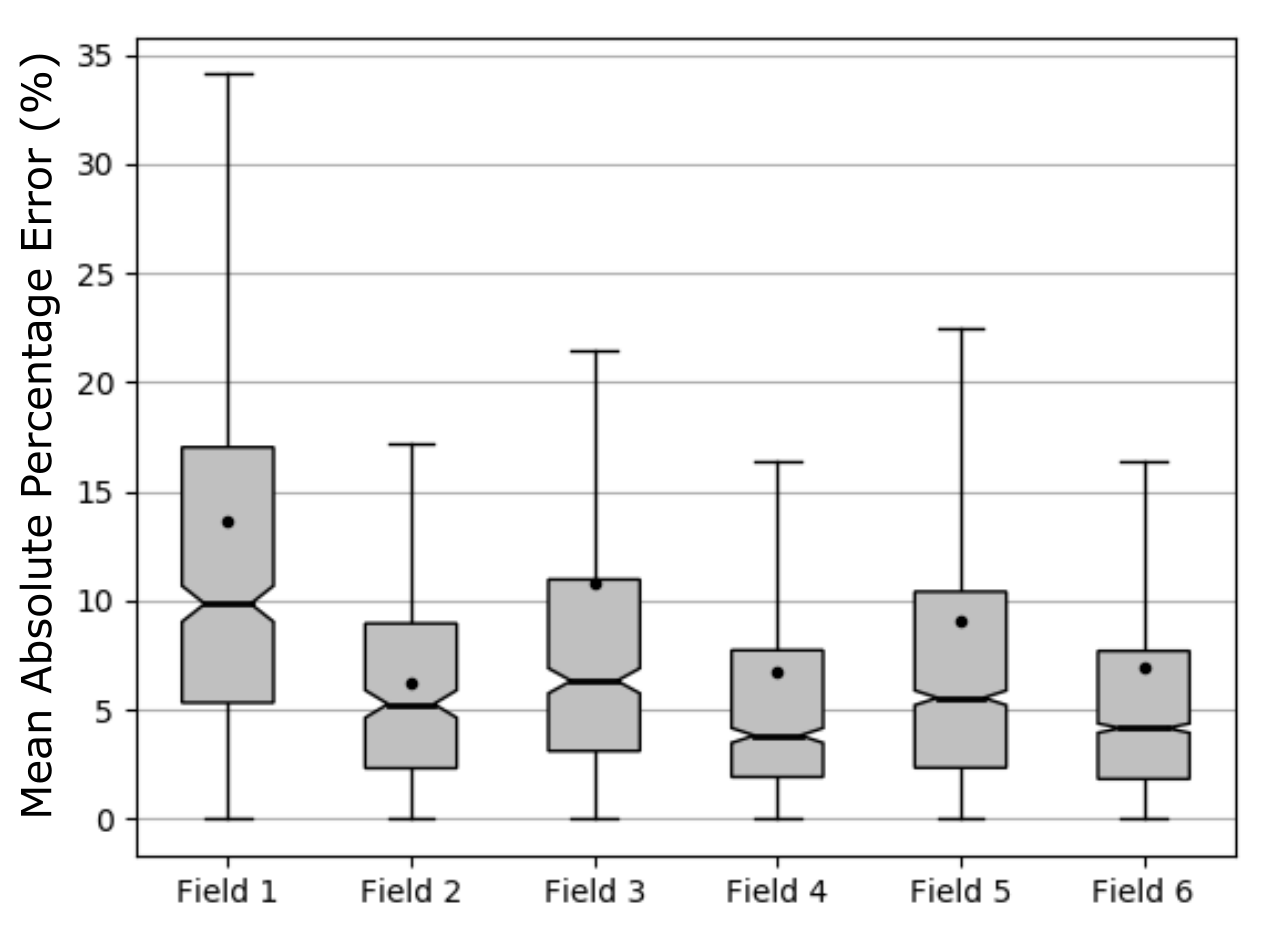
\includegraphics[width = 0.6\textwidth]{Images/ii-MAPE_boxplots.png}
    \caption{Boxplots of percentage error between true yield and predicted yield for each field (reproduced from [II]).}
    \label{fig:ii-boxplots}
\end{figure}

The model was also designed to be utilized as an AI engine in an Oskari-based (\emph{www.oskari.org}, MIT \& EUPL licensed) geospatial data mapping and farming decision support system. Through the web portal farmers can access their personal, authenticated accounts, upload data for visualization and call on AI based analytical tools for decision support.

\subsection{Sequence of inputs to single target}
\label{subsec:sequence-input-results}

In [IV] we examined the effect of time, as an additional feature, on intra-field yield prediction. Especially, capabilities of deep learning time series models utilizing UAV remote sensing time series data as their inputs were focused on. The objectives were two-fold: to see if the performance of the point-in-time model of [I] could be surpassed using spatiotemporal deep learning model architectures and to see which spatiotemporal architecture would perform better in the same task. The usability of spatiotemporal models was evaluated in two settings, end-of-season (full sequence) and in-season (limited sequence) prediction. Three model architectures were designed, trained and evaluated: a CNN-LSTM \cite{Sainath2015}, a convolutional LSTM \cite{Shi2015a} and a 3D-CNN \cite{Tran2015}. These models utilize the properties of CNNs and LSTM networks them to perform spatiotemporal modelling. The main contribution of the study was to perform time series based intra-field yield prediction with multi-temporal data collected during the growing season with UAVs.

Nine crop fields totaling to approximately 85 ha and having wheat, barley and oats as the crop varieties, were included in the study. The field-wise data was acquired during year 2018 in the proximity of Pori, Finland (61$^\circ$29'6.5''N, 21$^\circ$47'50.7''E). Specific information about the fields is given in Table~\ref{tab:iv-field-info}. The acquisition of input and target data was similar to [I]. 

\begin{table}[ht]
    \scriptsize
    \centering
    \caption{The fields selected for the multitemporal study in the proximity of Pori, Finland (reproduced from [IV]).}
    \label{tab:iv-field-info}
    \vspace{0.3cm}
    \begin{tabular}{@{}cccccc@{}}
    \toprule
    \textbf{\makecell{Field\\\#}} & \textbf{\makecell{Size \\ (ha)}} & \textbf{\makecell{Mean yield \\ (kg/ha)}} & \textbf{\makecell{Crop\\(\textit{Variety})}} & \textbf{\makecell{Thermal\\time}} & \textbf{\makecell{Sowing\\date}} \\ \midrule
    1                             & 11.11                            & 4349.1                                    & \makecell{Wheat\\(\textit{Mistral})}         & 1290.3                            & 13 May                           \\
    2                             & 7.59                             & 5157.6                                    & \makecell{Wheat\\(\textit{Mistral})}         & 1316.8                            & 14 May                           \\
    3                             & 11.77                            & 5534.3                                    & \makecell{Barley\\(\textit{Zebra})}          & 1179.9                            & 12 May                           \\
    4                             & 11.08                            & 3727.5                                    & \makecell{Barley\\(\textit{Zebra})}          & 1181.3                            & 11 May                           \\
    5                             & 7.88                             & 4166.9                                    & \makecell{Barley\\(\textit{RGT Planet})}     & 1127.6                            & 16 May                           \\
    6                             & 13.05                            & 4227.9                                    & \makecell{Barley\\(\textit{RGT Planet})}     & 1117.1                            & 19 May                           \\
    7                             & 7.61                             & 6668.5                                    & \makecell{Oats\\(\textit{Ringsaker})}        & 1223.4                            & 17 May                           \\
    8                             & 7.77                             & 5788.2                                    & \makecell{Barley\\(\textit{Harbringer})}     & 1136.1                            & 21 May                           \\
    9                             & 7.24                             & 6166.0                                    & \makecell{Oats\\(\textit{Ringsaker})}        & 1216.4                            & 18 May                           \\ \bottomrule
    \end{tabular}
\end{table}

Images of the fields were acquired with a SEQUIOA (Parrot Drone SAS, Paris, France) multispectral camera mounted on a Airinov Solo 3DR (Parrot Drone SAS, Paris, France) UAV on a weekly basis for 15 consecutive weeks. To encode passing of time for the temporal models, weather data was acquired from the open interface provided by the Finnish Meteorological Institute for Pori area. Being a common way to express crop growth phase, the cumulative temperature was utilized as the temporal feature in the input data. Temporally varying but spatially constant cumulative temperature was added as an additional layer in conjunction with the RGB layers to have the data contain necessary information for temporal feature learning. The targets data, crop yields, were acquired during the harvest of each field. The harvesters were equipped with either a Trimble Navigation (Sunnyvale, California, USA) CFX 750 or John Deere (Moline, Illinois, USA) Greenstar 1 yield mapping sensor systems, which produce a cloud of geolocated points with multivariate information about the harvest for each point in vector format.

The fields were split into smaller overlapping frames of size 40 $\times$ 40 m with a lateral and vertical step of 10 m. Sequences of frames of fixed width and height were extracted from sequences of field plot images and corresponding weather data as the input data. The input frames were then geolocationally paired with corresponding yield data to form input-target pairs. A total of 2586 sequences, 15 geolocationally matching frame rasters per sequence, were extracted from the data. Lastly, data was shuffled and split to training and test sets with a 70\%/30\% ratio, respectively. The general process of generating the frames is depicted in Figure~\ref{fig:iv-data-processing}.

\begin{figure}[htb]
    \centering
    \includegraphics[width = 0.8\textwidth]{images/iv-data-processing.png}
    \caption{Input frame sequence and target average yield extraction process (reproduced from [IV]).} 
    \label{fig:iv-data-processing}
\end{figure}

All models we trained with random search \cite{Bergstra2012}. For the CNN-LSTM, the CNN of the model was first trained separately with distinct frames, i.e. point-in-time data. Training the model from scratch was required due to changes in input channel count. It was trained according to the best results of [I], using Adadelta \cite{Zeiler2012} as the optimizer. For the spatiotemporal models, Adam \cite{Kingma2015} was used as the optimizing algorithm for each model architecture akin to \cite{Rustowicz2019}, \cite{Yaramasu2020} and \cite{Liu2017}. The spatiotemporal models were trained with frame sequences. A total of 950 models were trained, with 300 for each spatiotemporal model and 50 for the CNN of the CNN-LSTM. 

In the first phase the models were trained to perform end-of-season predictions with full length frame sequences. The trained models were evaluated with a hold-out test set and the results are given in Table~\ref{tab:iv-test-results}. The number of trainable parameters indicate the model complexity and the best values are in bold. Best performance was achieved with the 3D-CNN architecture. 
 
% Please add the following required packages to your document preamble:
% \usepackage{booktabs}
\begin{table}[htb]
    \scriptsize
    \centering
    \caption{The end-of-season prediction performance metrics of the best spatiotemporal models (reproduced from [IV]).}
    \label{tab:iv-test-results}
    \vspace{0.3cm}
    \begin{tabular}{@{}llllll@{}}
    \toprule
    \textbf{Model} & \textbf{\begin{tabular}[c]{@{}l@{}}Test RMSE\\(kg/ha)\end{tabular}} & \textbf{\begin{tabular}[c]{@{}l@{}}Test MAE\\(kg/ha)\end{tabular}} & \textbf{\begin{tabular}[c]{@{}l@{}}Test MAPE\\(\%)\end{tabular}} & \textbf{\begin{tabular}[c]{@{}l@{}}Test R$^2$\\ -\end{tabular}} & \textbf{\begin{tabular}[c]{@{}l@{}}Trainable\\ parameters\end{tabular}} \\ \midrule
    Pretrained CNN & 692.8                                                               & 472.7                                                              & 10.95                                                            & 0.780                                                           & 2.72$\times 10^{6}$                                                     \\
    CNN-LSTM       & 456.1                                                               & 329.5                                                              & 7.97                                                             & 0.905                                                           & 2.94$\times 10^{6}$                                                     \\
    ConvLSTM       & 1190.3                                                              & 926.9                                                              & 22.47                                                            & 0.349                                                           & 9.03$\times 10^{5}$                                                     \\
    3D-CNN         & \textbf{289.5}                                                      & \textbf{219.9}                                                     & \textbf{5.51}                                                    & \textbf{0.962}                                                  & 7.48$\times 10^{6}$                                                     \\ \bottomrule
    \end{tabular}
\end{table}

In-season prediction performance was evaluated with the best performing 3D-CNN model configuration and using data from an actionable time frame from the beginning of the growing season. Multiple input data configuration were tested, forming varying sequences of 3 to 5 frames from five first weeks of imaging (weeks 21 to 25 of 2018). Overall, the best perfoming in-season sequence cconfiguration in terms of MAE was the four-week-long sequence taken from the beginning of the season (weeks 21 to 24) with 292.8 kg/ha MAE, 7.17 \% MAPE and 0.929 R$^2$. Visualized prediction results are illustrated in Figure~\ref{fig:iv-true-pred} with a 10 meter step between predicted points. 

\begin{figure}[htb]
    \centering
    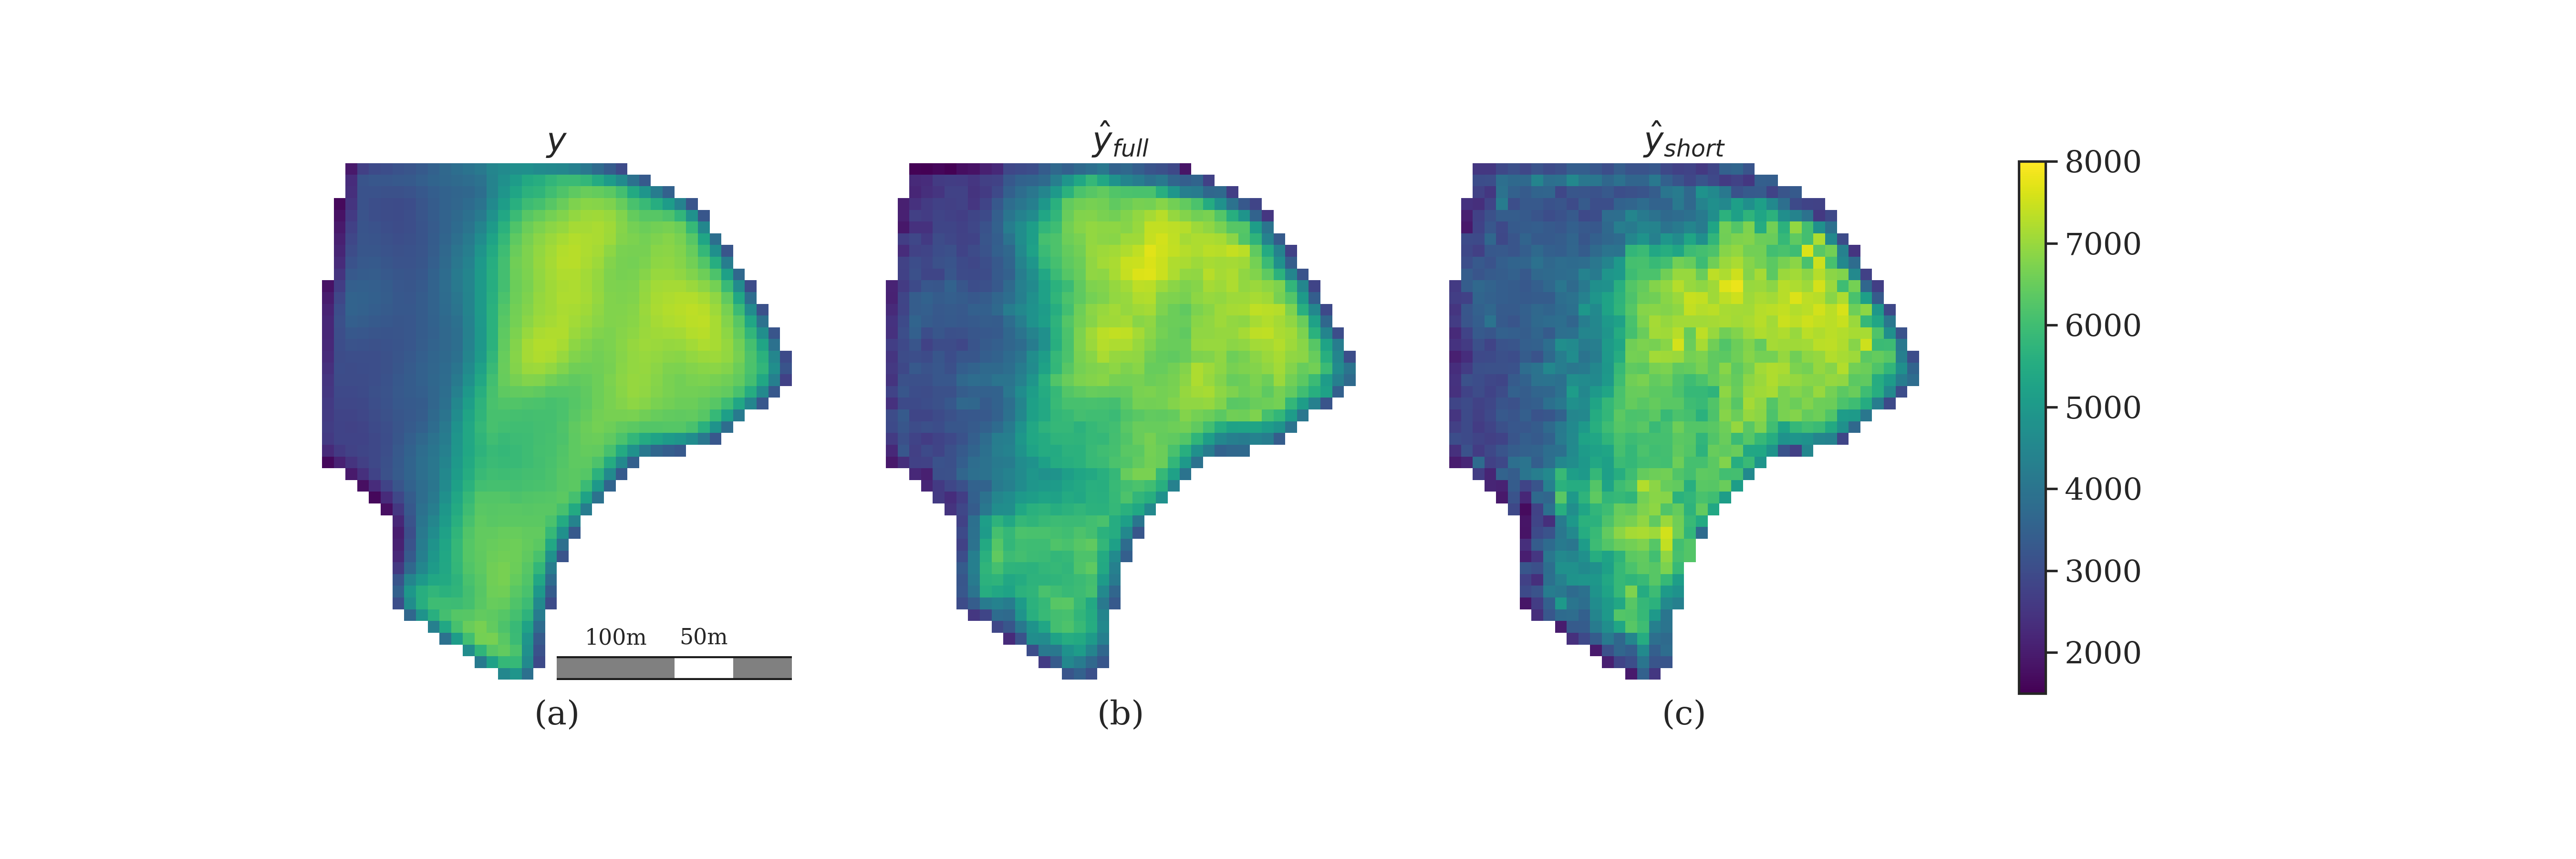
\includegraphics[width = \textwidth]{Images/iv-true_pred.png}
    \caption{Frame-based 3D-CNN model performances against true yield data (reproduced from [IV]).}
    \label{fig:iv-true-pred}
\end{figure}

\section{Remote sensing data evaluation}
\label{sec:input-assessment-results}


\subsection{Additional input sources}
\label{subsec:additional-inputs-results}

In [V] the effects of additional field-related spatial or spatial-like data on the intra-field crop yield prediction capabilities were studied. The model architecture was taken from [I] and a baseline was trained with RGB data from the earlier half of the growing season of 2018 (weeks 21 to 26). The objective of the study was to assess crop yield prediction capabilities with the best CNN model composition from [I] by varying the input data configurations with additional data. Additional data sources included data from the following sources: local weather stations, soil samplings, soil sensors and Sentinel-2 satellite system. Disregarding the changing number of input channels, the architectural and optimizer related hyperparameters were not changed to better isolate the effects of different input configurations on the yield estimation performance.

Four crop fields were selected for data acquisition in the vicinity of Pori, Finland (61$^\circ$29'6.5''N, 21$^\circ$47'50.7''E) for the growing season of 2018. The field information is provided in Table~\ref{tab:v-field-info}. The multisource input data for the fields consists of UAV-based RGB images, multispectral Sentinel-2 \cite{ESAS2} satellite data, sparsely collected and analyzed soil samplings, machine-collected soil information, topography information and local weather station data. 

\begin{table}[htb]
    \scriptsize
    \centering
    \caption{The fields selected for multisource study in the proximity of Pori, Finland (reproduced from [V]).}
    \label{tab:v-field-info}
    \vspace{0.3cm}
    \begin{tabular}{@{}cccccc@{}}
    \toprule
    \textbf{\makecell{Field\\\#}} & \textbf{\makecell{Size \\ (ha)}} & \textbf{\makecell{Mean yield \\ (kg/ha)}} & \textbf{\makecell{Crop\\(\textit{Variety})}} & \textbf{\makecell{Thermal\\time ($^{\circ}$C)}} & \textbf{\makecell{Sowing\\date}} \\ \midrule
    1                             & 7.59                             & 5157.6                                    & \makecell{Wheat\\(\textit{Mistral})}         & 1316.8                            & 14 May                           \\
    2                             & 11.77                            & 5534.3                                    & \makecell{Barley\\(\textit{Zebra})}          & 1179.9                            & 12 May                           \\
    3                             & 7.88                             & 4166.9                                    & \makecell{Barley\\(\textit{RGT Planet})}     & 1127.6                            & 16 May                           \\
    4                             & 7.24                             & 6166.0                                    & \makecell{Oats\\(\textit{Ringsaker})}        & 1216.4                            & 18 May                           \\ \bottomrule
    \end{tabular}
\end{table}

General information about the original data sources are given in Table~\ref{tab:v-data-general}. UAV data was acquired with weekly overfligths of each field using a SEQUIOA (Parrot Drone SAS, Paris, France) multispectral camera mounted on a Airinov Solo 3DR (Parrot Drone SAS, Paris, France) UAV. The Sentinel-2 satellite data for the fields was acquired from the Copernicus Open Access Hub (European Space Agency, Paris, France), date-matched with UAV-images. Soil samples were collected manually during November 2018 from the fields with 50 m steps by ProAgria, an agronomic counseling instution, and sent to a Eurofins (Eurofins Viljavuuspalvelu, Mikkeli, Finland) laboratory for further analysis. An MSP3 soil scanner (Veris Technologies, Salina, Kansas, USA) was used to map the fields at depths of 0-30 cm and 30-90 cm. The measurements were performed during April and May of 2019. Lidar-based topographical information was acquired from the open-access data portal of the National Land Survey of Finland. Weather data was collected with two separately located Vantage Pro2 (Davis Instruments, Hayward, California, USA) weather stations. Yield data was acquired during the harvest of 2018 with yield mapping sensor devices attached to the harvesters, either with a CFX 750 (Trimble Navigation, Sunnyvale, California, USA) or Greenstar 1 (John Deere, Molinde, Illinois, USA). 

% Please add the following required packages to your document preamble:
% \usepackage{booktabs}
\begin{table}[htb]
    \centering
    \scriptsize
    \caption{General information of data sources and their original formats (reproduced from [V]).}
    \label{tab:v-data-general}
    \begin{tabular}{@{}lllll@{}}
    \toprule
    \textbf{Source} & \textbf{Type} & \textbf{Resolution/Step} & \textbf{Multitemporal} & \textbf{Channels} \\ \midrule
    UAV             & Raster        & 0.3125 m/px              & Yes                    & 3                 \\
    Sentinel-2     & Raster        & {[}10,20,60{]} m/px      & Yes                    & 19                \\
    Soil samples    & Vector        & 50 m                     & No                     & 8                 \\
    Veris MSP3      & Vector        & 20 m                     & No                     & 6                 \\
    Topography      & Vector        & 2 m                      & No                     & 1                 \\
    Weather         & Tabular       & -                        & Yes                    & 2                 \\
    Yield           & Vector        & Varying                  & No                     & 1                 \\ \bottomrule
    \end{tabular}
\end{table}

All inputs were harmonized to the spatial resolution of the RGB data, 0.3125~m/px by interpolating coarser data sources with GDAL utility's \texttt{gdal\_grid} program with \texttt{invdist:power=3:smoothing=20} interpolation algorithm. After that, overlapping frames were extracted from the data for each week, resulting in a total of 16375 frames. As the number of unique fields was low, maximizing the sample variability the model sees during training was necessary. The data was divided to distinct training, validation and test sets according to the UAV image acquisition week and shuffled to eliminate spatial autocorrelation in subsequent samples due to overlapping frame extraction. 

The last step of data processing was to build the data sets for different data source configurations. Four distinct configurations were considered:

\begin{itemize}
    \item \emph{RGB Only}, which uses UAV RGB data only
    \item \emph{No S2}, which uses UAV, soil, Veris MSP3, topography and weather data
    \item \emph{S2 Raw}, which adds Sentinel-2 raw wavelength band data to \emph{No S2}
    \item \emph{S2 Full}, which adds calculated Sentinel-2 Level-2A product layers to \emph{S2 Raw}.
\end{itemize}

Ten models were trained for each configuration to account for random initialization of the models inner parameters (weights) and the best models for each configuration were considered. The performance with larger number of fields using UAV RGB data has already been extensively studied in [I] and [IV]. Thus, training a model with only UAV RGB data provides a studied baseline to which models trained with additional data can be compared. The baseline model using UAV RGB data only attained 1055.7 kg/ha test RMSE, 18.2\% test MAPE and 0.343 test R$^2$. The best performing data configuration was \emph{S2 Full} with 364.1 kg/ha test RMSE, 5.18\% test MAPE and 0.922 test R$^2$ using all 39 layers of input data for each extracted frame. Compared to the baseline \emph{RGB Only} model, the \emph{S2 Full} attained 65.6\% lower RMSE, 67.3\% lower MAE, 71.5\% better MAPE and 0.579 higher R$^2$ with the test set. Generally every model with multisource inputs performed better than the baseline model. This is shown in Table~\ref{tab:v-relative-results}.

% Please add the following required packages to your document preamble:
% \usepackage{booktabs}
% \usepackage{multirow}
\begin{table}[htb]
    \scriptsize
    \centering
    \caption{The relative performance of the models trained with distinct multisource input data configurations to the baseline \emph{RGB Only} model (reproduced from [V]).}
    \label{tab:v-relative-results}
    \begin{tabular}{@{}lllll@{}}
    \toprule
    \multirow{2}{*}{\textbf{\begin{tabular}[c]{@{}l@{}}Data\\ Setting\end{tabular}}} & \multicolumn{4}{c}{\textbf{Relative change from \emph{RGB Only}}}                                                                                                                                                                                                                         \\
                                                                                     & \textbf{Test RMSE} & \textbf{Test MAE} & \textbf{Test MAPE} & \textbf{Test R$^2$} \\ \midrule
    No S2                                                                            & -15.5\%            & -17.2\%           & -18.7\%            & +0.188               \\
    S2 Raw                                                                           & -56.3\%            & -59.4\%           & -61.9\%            & +0.532               \\
    S2 Full                                                                          & \textbf{-65.6\%}   & \textbf{-67.3\%}  & \textbf{-71.5\%}   & \textbf{+0.579}      \\ \bottomrule
    \end{tabular}
\end{table}


\subsection{Satellite data reliability}
\label{subsec:satellite-quality-results}

Data from the Sentinel-2 satellites are intensively used for various applications such as land use and vegetation mapping or crop monitoring. Depending on climate conditions in the region of interest, one of the main obstacles in using the data for practical monitoring purposes is cloud coverage. Currently, the cloud mask of the Sentinel data is available in the form of the Level 1C product containing vector layers of dense and cirrus clouds. Also, the percentage of cloudy pixels (dense and cirrus) in the mask are provided. The Level 2A product further processes the Level 1C data to obtain the Scene Classification layer with cloud and cirrus probability values at 60 m spatial resolution. According to Coluzzi et.al. \cite{Coluzzi2018}, caution has to be taken when using the provided cloud masks and improved cloud detection algorithms are welcome.

Therefore, a random forest classifier was trained to assess cloud cover in Sentinel-2 data in [III], using data acquired from crop fields by UAVs as ground truth for cloudless data. For cloudless multispectral ground truth data, ten crop fields were selected for imaging during 2018 and 2019 in the vicinity of Pori, Finland (61$^\circ$29'N, 21$^\circ$48'E). The fields were imaged approximately weekly with two distinct drones both years, using 3DR Solo (Parrot Drone SAS, Paris, France) for the year 2018 and Disco-Pro AG (Parrot Drone SAS, Paris, France) for 2019. The drones were equipped with similar SEQUIOA (Parrot Drone SAS, Paris, France) multispectral cameras. Half of the fields had wheat (\textit{Zebra/Mistral}), three had barley (\textit{Harbringer/RGT Planet}) and two remaining had oats (\textit{Ringsaker}) as the cultivated crop. The total area of the selected fields was approximately 93 ha. The drone images were downsampled to match the highest resolution available in Sentinel-2 images, 10 m/px. In total, 288 images of distinct crop field images constituted the complete data set.

However, comparing absolute values across bands for two different sensors and imaging platforms proved out to be difficult, as the data would require scaling to an unkown global maximum for Sentinel-2. Thus, using the NDVI values calculated from both data sources (UAV and Sentinel-2) was deemed appropriate due to the index providing normalized and thus comparable data between distinct imaging systems.

To facilitate data based modelling in a supervised setting, target values are required. Due to UAV flight altitude of 150 m eters, Sentinel-2 data can be seen as being cloudless when the NDVI values for a field are similar to the UAV based values as possible. Thus, the task of classification is that of classifying Sentinel-2 data either similar or dissimilar to the UAV data. The similarity for a single pixel-corresponding area is determined by

\begin{equation}
    sim_{(s,d)} = \begin{cases}  1, & |s-d| \leq threshold \\ 
    0, & \mbox{otherwise} 
    \end{cases}
    \label{eq:iii-similarity}
\end{equation}

\noindent where $s$ and $d$ are spatially and temporally aligned NDVI pixels for a field from the satellite and drone sources respectively. Similarity indicates that Sentinel-2 data is cloudless, while dissimilarity indicates cloudiness. The threshold had to be determined via empirical analysis. The task of determining the threshold for labeling is a task of balancing between (1) capturing as much similarities while (2) still excluding as many dissimilarities as possible. Using Students $t$-test, a total of 15 statistically similar ($p = 0.01$) week-aligned NVDI image pairs were found. Usign similar images, the threshold of similarity was empirically determined by comparing the ratio of pixels deemed similar produced by various thresholds with Equation~\ref{eq:iii-similarity}. The threshold of 0.075 absolute difference in NDVI was selected. A single image pair with the calculated similarity map is shown in Fig.~\ref{fig:iii-s2-drone-comparison}. The first two figures depict the NDVI maps from corresponding sources. The third figure shows the absolute difference between the aligned Sentinel-2 and drone NDVI values. The fourth figure shows the thresholded absolute difference, indicating areas where the NDVI images are similar enough. 

\begin{figure*}[htb]
    \centering
    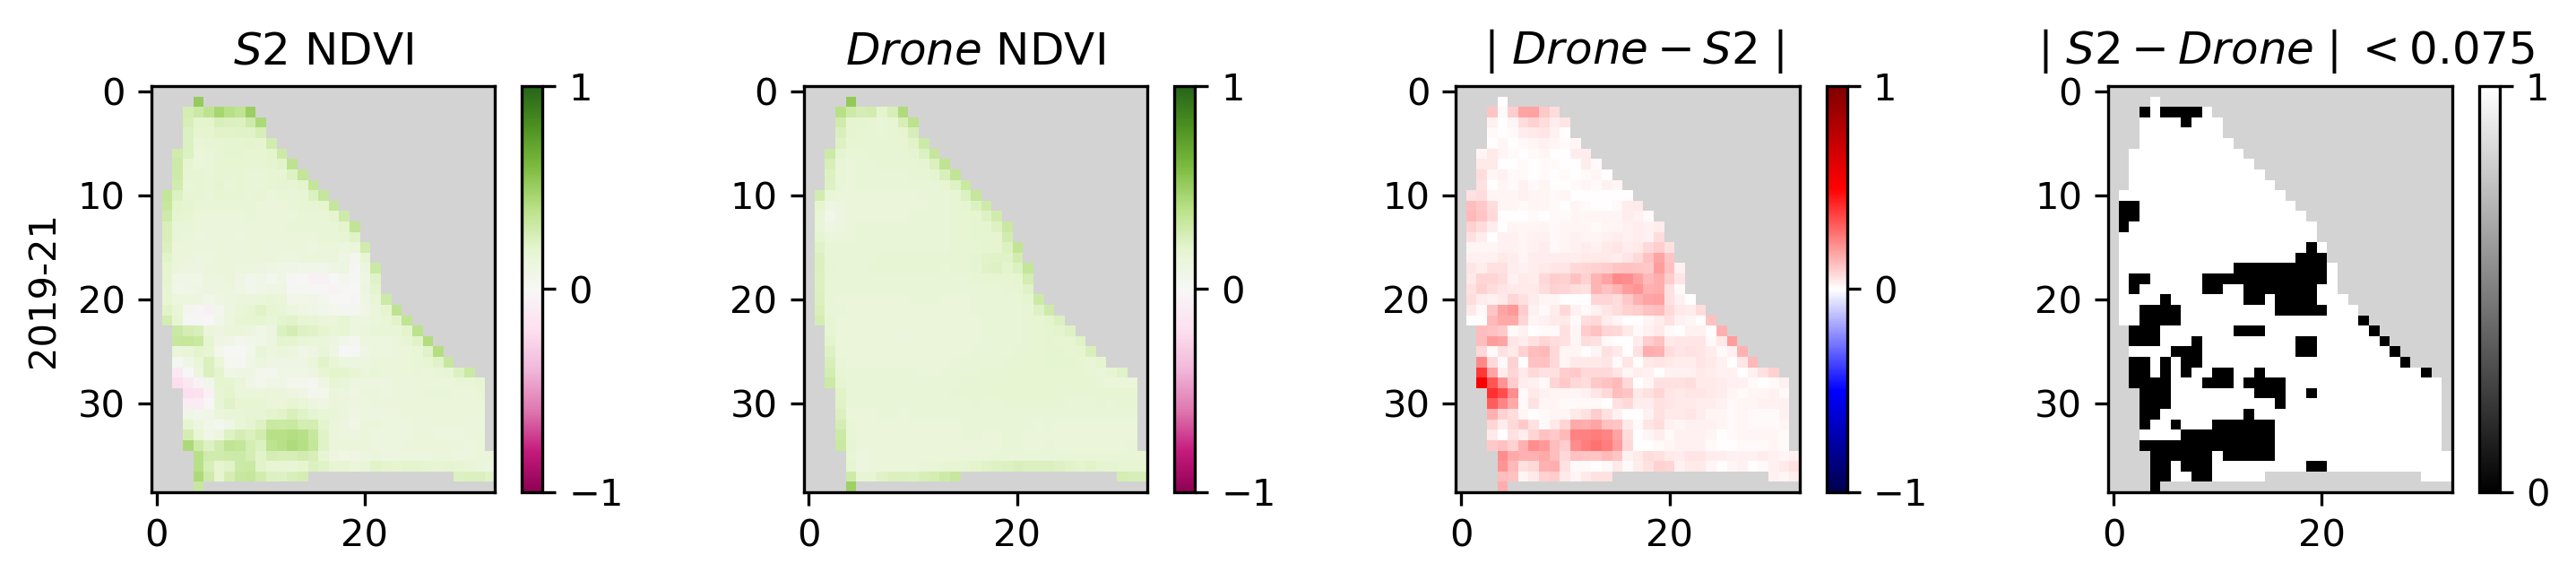
\includegraphics[width=\textwidth]{./Images/iii-targets-8860198450-2019-21.png}
    \caption{A visualization of a single week-aligned Sentinel-2 and drone NDVI image pair with the absolute difference and the similarity map (reproduced from [III]).}
    \label{fig:iii-s2-drone-comparison}
\end{figure*}

\begin{table}[htb]
    \centering
    \scriptsize
    \caption{The confusion matrix of similarity label predictions (reproduced from [III]).}
    \label{tab:iii-confusion-matrix}
    \begin{tabular}{@{}ccc@{}}
    \toprule
    Pred/True  & \textbf{0}                                                              & \textbf{1}                                         \\ \midrule
    \textbf{0} & \multicolumn{1}{c|}{\begin{tabular}[c]{@{}c@{}}TP\\ 23237\end{tabular}} & \begin{tabular}[c]{@{}c@{}}FP\\ 2580\end{tabular}  \\ \cmidrule(l){2-3} 
    \textbf{1} & \multicolumn{1}{c|}{\begin{tabular}[c]{@{}c@{}}FN\\ 1807\end{tabular}}  & \begin{tabular}[c]{@{}c@{}}TN\\ 36037\end{tabular} \\ \bottomrule
    \end{tabular}
\end{table}

\begin{table}[htb]
    \centering
    \scriptsize
    \caption{Similarity estimates with hold out test data (reproduced from [III]).}
    \label{tab:iii-model-s2-comparison}
    \begin{tabular}{@{}lllllll@{}}
    \toprule
                                 & \multicolumn{3}{c}{$y = 0$}                         & \multicolumn{3}{c}{$y = 1$}     \\
                                 & Mean          & Std   & Median                   & Mean          & Std  & Median \\ \midrule
    Model                        & \textbf{0.07} & 0.25 & \multicolumn{1}{l|}{0.00} & 0.93          & 0.26 & 1.00  \\
    $\text{CLDPRB}_{\text{SIM}}$ & 0.45          & 0.45 & \multicolumn{1}{l|}{0.26} & \textbf{0.97} & 0.14 & 1.00  \\
    $\text{SCL}_{\text{SIM}}$    & 0.28          & 0.45 & \multicolumn{1}{l|}{0.00} & 0.95          & 0.22 & 1.00  \\ \midrule
    Samples                      & \multicolumn{3}{c}{38617}                           & \multicolumn{3}{c}{25044}       \\ \bottomrule
    \end{tabular}
\end{table}

The thresholded binary value maps constitute the target data for pixel-wise binary classification, while Sentinel-2 data was used as inputs. A total of 381972 input-target samples (pixels) were extracted from the source data. The samples were then shuffled and split into training and test data sets with 190986 and 63661 samples, correspondingly. Due to using data in tabular manner, where an input pixel contains several values and spatial dependencies are not modelled, a decision tree based random forest was deemed an appropriate model to use. The confusion matrix of model predictions against true labels with test data is shown in Table~\ref{tab:iii-confusion-matrix}.

The comparison of sample-wise similarity estimations between the trained model and Sentinel-2 data products are given in Table~\ref{tab:iii-model-s2-comparison}. The estimates are given both for when the true target value was 0 (satellite differed from drone) and when it was 1 (satellite similar to drone). For cloudless Sentinel-2 data, the model performed close to existing cloudiness estimates provided with the data products. For cloudy data, the model performed significantly better.

